\section{Các lệnh đã thiết lập}
\subsection{Lệnh sleep}
\underline{\textbf{Chức năng của lệnh:}} Lệnh \verb|sleep <number of ticks>| cho phép người dùng dừng hệ thống trong số ticks nhất định (\textbf{ticks} là một đơn vị thời gian được quy định trong hệ điều hành xv6) \cite{mit-xv6}.

\underline{\textbf{Thiết lập thuật toán:}} Gọi hàm \verb|sleep| từ thư viện \verb|user.h| được cung cấp sẵn trong xv6 và chuyển chuỗi số trong câu lệnh về kiểu số nguyên. Lệnh sẽ báo lỗi khi nhập sai cú pháp.

Dưới đây là kết quả chạy thử trên \verb|qemu| và kiểm tra lệnh \verb|sleep| bằng chương trình kiểm thử:
\begin{figure}[htp!]
	\centering
	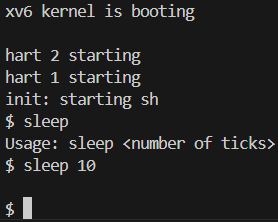
\includegraphics[width=0.5\textwidth]{figures/exec-sleep}
	\caption{Kết quả chạy thử \textbf{sleep} trên \textbf{qemu}}
\end{figure}
\begin{figure}[htp!]
	\centering
	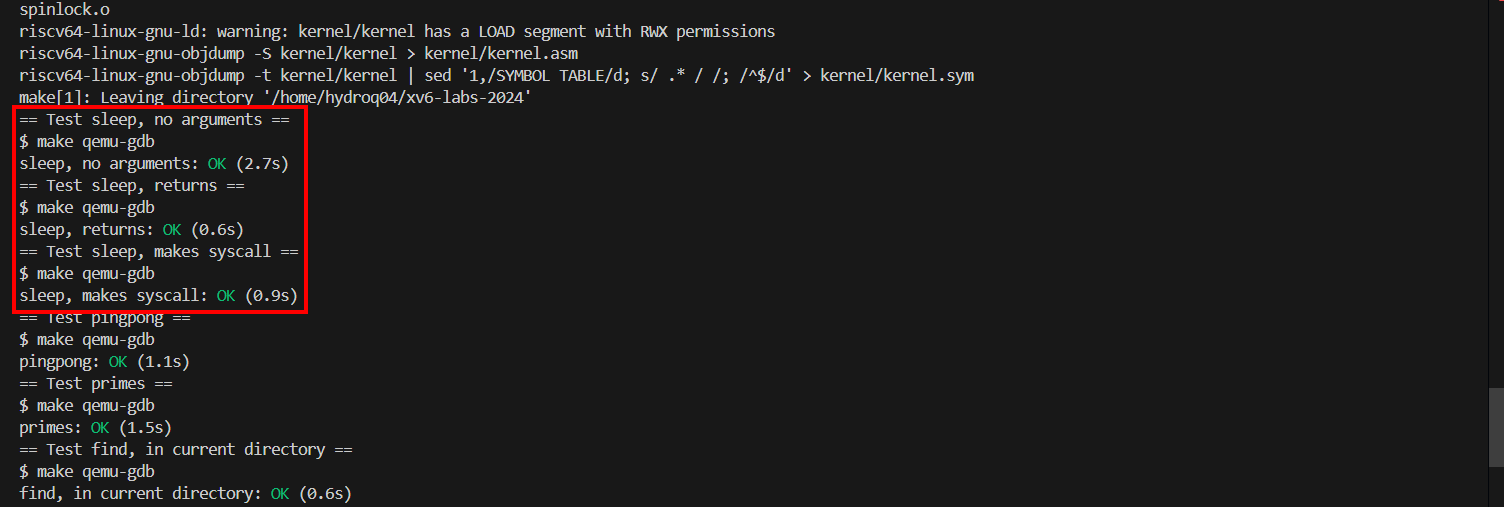
\includegraphics[width=0.9\textwidth]{figures/sleep-test}
	\caption{Kết quả kiểm thử \textbf{sleep} bằng công cụ chấm bài \textbf{grade} của MIT}
\end{figure}

\newpage